% !TEX enableShellEscape = yes
% (The above line makes atom's latex package compile with -shell-escape
% for minted, and is just ignored by other systems.)
\documentclass{article}

\usepackage{fullpage}
\usepackage{color}
\usepackage{amsmath,amssymb}
\usepackage{url}
\usepackage{verbatim}
\usepackage{graphicx}
\usepackage{parskip}
\usepackage{amssymb}
\usepackage{hyperref}

% Use one or the other of these for displaying code.
% NOTE: If you get
%  ! Package minted Error: You must invoke LaTeX with the -shell-escape flag.
% and don't want to use minted, just comment out the next line
\usepackage{minted} \BeforeBeginEnvironment{minted}{\begingroup\color{black}} \AfterEndEnvironment{minted}{\endgroup} \setminted{autogobble,breaklines,breakanywhere,linenos}

\usepackage{listings}

% Colours
\definecolor{blu}{rgb}{0,0,1}
\newcommand{\blu}[1]{{\textcolor{blu}{#1}}}
\definecolor{gre}{rgb}{0,.5,0}
\newcommand{\gre}[1]{\textcolor{gre}{#1}}
\definecolor{red}{rgb}{1,0,0}
\newcommand{\red}[1]{\textcolor{red}{#1}}
\definecolor{pointscolour}{rgb}{0.6,0.3,0}

% answer commands
\newcommand\ans[1]{\par\gre{Answer: #1}}
\newenvironment{answer}{\par\begingroup\color{gre}Answer: }{\endgroup}
\let\ask\blu
\let\update\red
\newenvironment{asking}{\begingroup\color{blu}}{\endgroup}
\newcommand\pts[1]{\textcolor{pointscolour}{[#1~points]}}

% Math
\def\R{\mathbb{R}}
\DeclareMathOperator*{\argmax}{arg\,max}
\DeclareMathOperator*{\argmin}{arg\,min}
\newcommand{\norm}[1]{\lVert #1 \rVert}
\newcommand{\mat}[1]{\begin{bmatrix}#1\end{bmatrix}}

% LaTeX
\newcommand{\fig}[2]{\includegraphics[width=#1\textwidth]{#2}}
\newcommand{\centerfig}[2]{\begin{center}\includegraphics[width=#1\textwidth]{#2}\end{center}}

\begin{document}

\title{CPSC 340 Assignment 5}
\date{}
\maketitle
\vspace{-6em}



\section*{Important: Submission Format \pts{5}}

Please make sure to follow the submission instructions posted on the course website.
\ask{We will deduct marks if the submission format is incorrect, or if you're not using \LaTeX{} and your submission is \emph{at all} difficult to read} -- at least these 5 points, more for egregious issues.
Compared to assignment 1, your name and student number are no longer necessary (though it's not a bad idea to include them just in case, especially if you're doing the assignment with a partner).

\vspace{1em}



\section{Kernel Logistic Regresion \pts{22}}

If you run \verb|python main.py -q 1| it will load a synthetic 2D data set, split it into train/validation sets, and then perform regular logistic regression and kernel logistic regression (both without an intercept term, for simplicity). You'll observe that the error values and plots generated look the same, since the kernel being used is the linear kernel (i.e., the kernel corresponding to no change of basis). Here's one of the two identical plots:
\centerfig{0.5}{figs/logReg.png}


\subsection{Implementing kernels \pts{8}}

Inside \texttt{kernels.py}, you will see classes named \texttt{PolynomialKernel} and \texttt{GaussianRBFKernel}, whose \verb|__call__| methods are yet to be written.
\begin{asking}
  Implement the polynomial kernel and the RBF kernel for logistic regression.
  Report your training/validation errors and submit the plots from \verb|utils.plot_classifier| for each case.
\end{asking}
You should use the kernel hyperparameters $p=2$ and $\sigma=0.5$ respectively,
and $\lambda=0.01$ for the regularization strength.
For the Gaussian kernel, please do \emph{not} use a $1/\sqrt{2\pi\sigma^2}$ multiplier.

\begin{answer}
	\begin{table}
		\centering
		\begin{tabular}{lll}
			\hline 
			& Polynomial & RBF  \\
			\hline 
			Training Error & 19.3\% & 13\%   \\
			Validation Error & 15\% &  9\%  \\
			\hline \\
		\end{tabular}
		\caption{Errors}
	\end{table}

	\begin{figure}
		\centering
		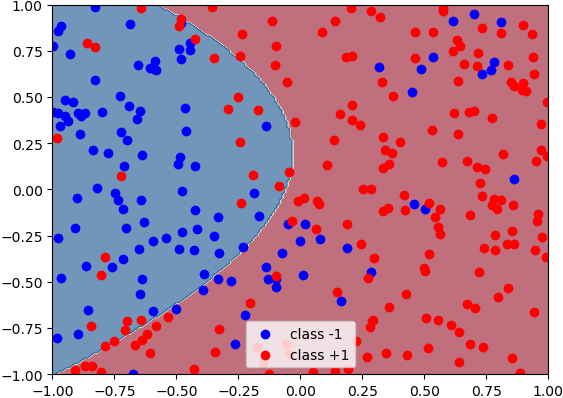
\includegraphics[width = .5\textwidth]{figs/logRegPoly.png}
		\caption{Polynomial Kernal Regression}
	\end{figure}


	\begin{figure}
		\centering
		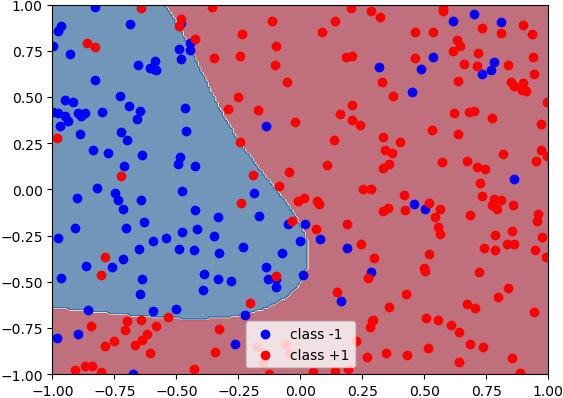
\includegraphics[width = .5\textwidth]{figs/logRegRBF.png}
		\caption{RBF Kernal Regression}
	\end{figure}


\end{answer}



\subsection{Hyperparameter search \pts{10}}

For the RBF kernel logistic regression, consider the hyperparameter values $\sigma=10^m$ for $m=-2,-1,\ldots,2$ and $\lambda=10^m$ for $m=-4,-3,\ldots,2$.
The function \verb|q1_2()| has a little bit in it already to help set up to run a grid search over the possible combination of these parameter values.
You'll need to fill in the \verb|train_errs| and \verb|val_errs| arrays
with the results on the given training and validation sets, respectively;
then the code already in the function will produce a plot of the error grids.
\ask{Submit this plot}.
Also, for each of the training and testing errors,
pick the best (or one of the best, if there's a tie) hyperparameters for that error metric,
and \ask{report the parameter values and the corresponding error, as well as a plot of the decision boundaries (plotting only the training set)}.
While you're at it, \ask{submit your code}.
To recap, for this question you should be submitting:
two decision boundary plots,
the values of two hyperparameter pairs with corresponding errors,
and your code.

Note: on the real job you might choose to use a tool like scikit-learn's \texttt{GridSearchCV} to implement the grid search, but here we are asking you to implement it yourself, by looping over the hyperparameter values.
\begin{answer}
	\begin{table}[htbp!]
		\centering
		\begin{tabular}{lcc}
			\hline 
			& Training & Validation   \\
			\hline 
			Best Sigma & 0.01 & 0.1   \\
			Best Lammy & 0.0001 &  1\\
			Best Error & 0 & 0.12 \\
			\hline \\
		\end{tabular}
		\caption{Best Parameters}
	\end{table}

	\begin{figure}[htbp!]
		\centering
		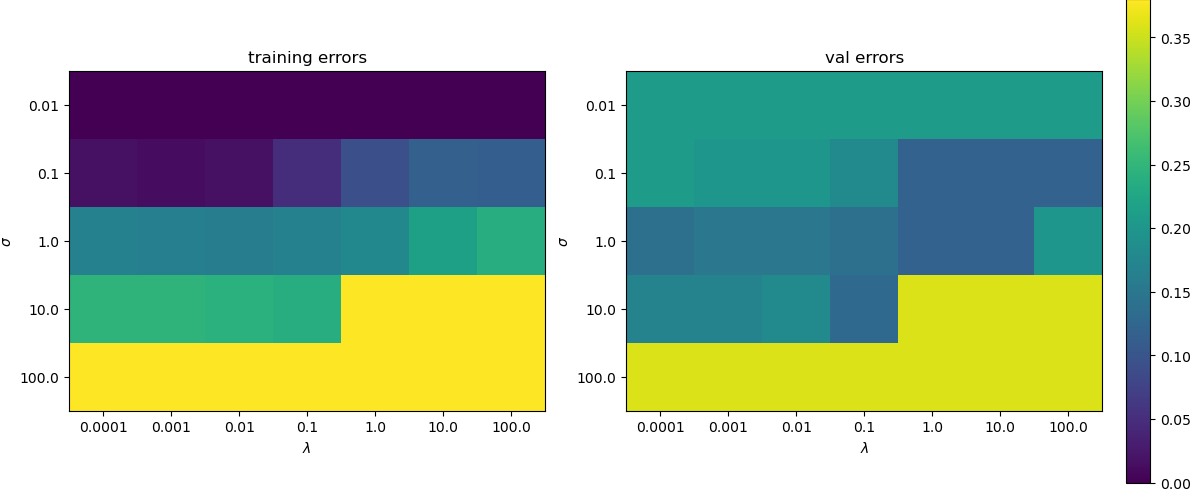
\includegraphics[width =  \textwidth]{figs/logRegRBF_grids.png}
		\caption{Error Grids}
	\end{figure}

	\begin{figure}[htbp!]
		\centering
		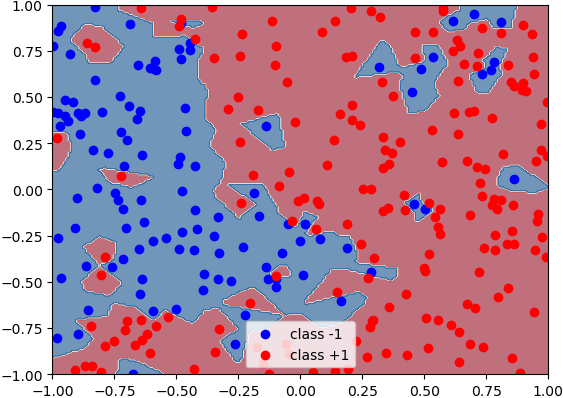
\includegraphics[width = .5\textwidth]{figs/best_train.png}
		\caption{Model with Best Training Error}
	\end{figure}

	\begin{figure}[htbp!]
		\centering
		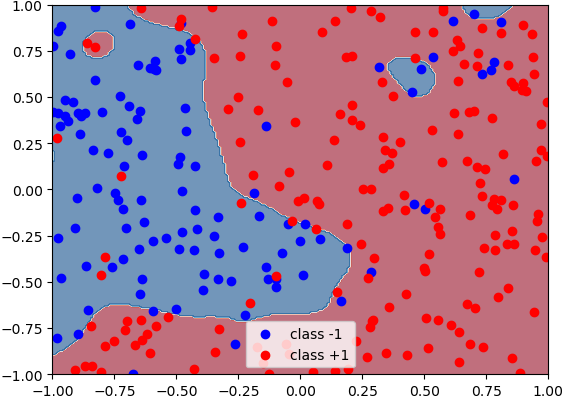
\includegraphics[width = .5\textwidth]{figs/best_val.png}
		\caption{Model with Best Validation Error}
	\end{figure}
	
	\clearpage

	\begin{minted}{python}
		#Find the best parameters	
		best_train_err = 100
		best_val_err = 100
		best_train_sigma = sigmas[0]
		best_train_lammy = lammys[0]
		best_val_sigma = sigmas[0]
		best_val_lammy = lammys[0]

		for i in range(5):
			for j in range(7):
				sigma_i = sigmas[i]
				lammy_j = lammys[j]
				loss_fn = KernelLogisticRegressionLossL2(lammy_j)
				optimizer = GradientDescentLineSearch()
				kernel = GaussianRBFKernel(sigma_i)
				klr_model = KernelClassifier(loss_fn, optimizer, kernel)
				klr_model.fit(X_train, y_train)

				train_errs[i,j] = np.mean(klr_model.predict(X_train) != y_train)
				val_errs[i,j] = np.mean(klr_model.predict(X_val) != y_val)

				if train_errs[i,j] < best_train_err:
					best_train_err = train_errs[i,j]
					best_train_sigma = sigmas[i]
					best_train_lammy = lammys[j]
				
				if val_errs[i,j] < best_val_err:
					best_val_err = val_errs[i,j]
					best_val_sigma = sigmas[i]
					best_val_lammy = lammys[j]


		#Print the best parameters        
		print("best training error: {:.5f}".format(best_train_err))
		print("lammy for best training error: {:.5f}".format(best_train_lammy))
		print("sigma for best training error: {:.5f}".format(best_train_sigma))

		print("best validation error: {:.5f}".format(best_val_err))
		print("lammy for best validation error: {:.5f}".format(best_val_lammy))
		print("sigma for best validation error: {:.5f}".format(best_val_sigma))

		#Plot the classification using the best train parameters
		loss_fn = KernelLogisticRegressionLossL2(best_train_lammy)
		optimizer = GradientDescentLineSearch()
		kernel = GaussianRBFKernel(best_train_sigma)
		klr_model = KernelClassifier(loss_fn, optimizer, kernel)
		klr_model.fit(X_train, y_train)
		fig = utils.plot_classifier(klr_model, X_train, y_train)
		utils.savefig("best_train.png", fig)

		#Plot the classification using the best validation parameters
		loss_fn = KernelLogisticRegressionLossL2(best_val_lammy)
		optimizer = GradientDescentLineSearch()
		kernel = GaussianRBFKernel(best_val_sigma)
		klr_model = KernelClassifier(loss_fn, optimizer, kernel)
		klr_model.fit(X_train, y_train)
		fig = utils.plot_classifier(klr_model, X_train, y_train)
		utils.savefig("best_val.png", fig)
	\end{minted}
	
\end{answer}


\subsection{Reflection \pts{4}}
\ask{
Briefly discuss the best hyperparameters you found in the previous part, and their associated plots. Was the training error minimized by the values you expected, given the ways that $\sigma$ and $\lambda$ affect the fundamental tradeoff?
}
\begin{answer}
	The parameter selections are reasonalbe. As $\lambda$ goes smaller, the classification becomes less regularization, and as $\sigma$ goes smaller, the model becomes more complex. Both way lead to overfitting problem, lowering the training error but increasing the approximation error.
\end{answer}


\clearpage
\section{MAP Estimation \pts{16}}

In class, we considered MAP estimation in a regression model where we assumed that:
\begin{itemize}
\item The likelihood $p(y_i \mid x_i, w)$ comes from a normal density with a mean of $w^Tx_i$ and a variance of $1$.
\item The prior for each variable $j$, $p(w_j)$, is a normal distribution with a mean of zero and a variance of $\lambda^{-1}$.
\end{itemize}
Under these assumptions, we showed that this leads to the standard L2-regularized least squares objective function,
\[
f(w) = \frac{1}{2}\norm{Xw - y}^2 + \frac \lambda 2 \norm{w}^2,
\]
which is the negative log likelihood (NLL) under these assumptions (ignoring an irrelevant constant).
\ask{For each of the alternate assumptions below, show the corresponding loss function} \pts{each 4}. Simplify your answer as much as possible, including possibly dropping additive constants.
\begin{enumerate}

\item We use a Gaussian likelihood where each datapoint has its own variance $\sigma_i^2$, and a zero-mean Laplace prior with a variance of $\lambda^{-1}$.
\[
p(y_i \mid x_i,w) = \frac{1}{\sqrt{2\sigma_i^2\pi}}\exp\left(-\frac{(w^Tx_i - y_i)^2}{2\sigma_i^2}\right), \quad p(w_j) = \frac{\lambda}{2}\exp(-\lambda|w_j|).
\]
You can use $\Sigma$ as a diagonal matrix that has the values $\sigma_i^2$ along the diagonal.

\begin{answer}
	\begin{equation*}
		f(w) = \frac{1}{2}(Xw - y)^T \Sigma^{-1} (Xw - y) + \lambda \norm{w}_1
	\end{equation*} 
\end{answer}

\item We use a Laplace likelihood with a mean of $w^Tx_i$ and a variance of $8$, and we use a zero-mean Gaussian prior with a variance of $\sigma^2$:
\[
p(y_i \mid x_i, w) = \frac14 \exp\left(- \frac12 |w^Tx_i - y_i| \right), \quad
p(w_j) = \frac{1}{\sqrt{2\pi} \, \sigma} \exp\left(-\frac{w_j^2}{2\sigma^2} \right).
\]

\begin{answer}
	\begin{equation*}
		f(w) = \frac{1}{2} \norm{Xw - y}_1 + \frac{1}{2 \sigma ^2} w^T w
	\end{equation*}
\end{answer}

 \item We use a (very robust) student $t$ likelihood with a mean of $w^Tx_i$ and $\nu$ degrees of freedom, and a Gaussian prior with a mean of $\mu_j$ and a variance of $\lambda^{-1}$,
\[
  p(y_i \mid x_i, w) = \frac{\Gamma\left(\frac{\nu + 1}{2}\right)}{\sqrt{\nu\pi}\Gamma\left(\frac \nu 2\right)}
                       \left(1 + \frac{(w^T x_i - y_i)^2}{\nu} \right)^{-\frac{\nu+1}{2}}
, \quad
  p(w_j) = \sqrt{\frac{\lambda}{2\pi}} \exp\left( -\frac\lambda2 (w_j - \mu_j)^2 \right).
\]
where $\Gamma$ is the \href{https://en.wikipedia.org/wiki/Gamma_function}{gamma function} (which is always non-negative).
You can use $\mu$ as a vector whose components are $\mu_j$.
\begin{answer}
	\begin{equation*}
		f(w) = \frac{\nu + 1}{2} \sum_{i = 1}^n \text{log} \left(1 + \frac{(w^T x_i - y_i)^2}{\nu}\right) + \frac{\lambda}{2} \norm{w - \mu}^2
	\end{equation*}
\end{answer}

\item We use a Poisson-distributed likelihood (for the case where $y_i$ represents counts), and a uniform prior for some constant $\kappa$,
\[
p(y_i | w^Tx_i) = \frac{\exp(y_iw^Tx_i)\exp(-\exp(w^Tx_i))}{y_i!}, \quad p(w_j) \propto \kappa.
\]
(This prior is 	``improper'', since $w\in\R^d$ but $\kappa$ doesn't integrate to 1 over this domain. Nevertheless, the posterior will be a proper distribution.)
\begin{answer}
	\begin{equation*}
		f(w) = \sum_{i = 1}^n \left(-y_i w^T x_i + \text{exp}(w^T x_i)\right)
	\end{equation*}
\end{answer}

\end{enumerate}


\clearpage
\section{Principal Component Analysis \pts{19}}
\subsection{PCA by Hand \pts{6}}

Consider the following dataset, containing 5 examples with 3 features each:
\begin{center}
  \begin{tabular}{ccc}
    $x_1$ & $x_2$ & $x_3$ \\
    \hline
     0 &  2 &  0 \\
     3 & -4 &  3 \\
     1 &  0 &  1 \\
    -1 &  4 & -1 \\
     2 & -2 &  2 \\
  \end{tabular}
\end{center}
Recall that with PCA we usually assume we centre the data before applying PCA (so it has mean zero).
We're also going to use the usual form of PCA where the PCs are normalized ($\norm{w} = 1$),
and the direction of the first PC is the one that minimizes the orthogonal distance to all data points.
\update{We're only going to consider $k = 1$ component here.}
\begin{enumerate}
  \item \ask{What is the first principal component?}
  \item \ask{What is the reconstruction loss (L2 norm squared) of the point $(2.5, -3, 2.5)$? (Show your work.)}
  \item \ask{What is the reconstruction loss (L2 norm squared) of the point $(1, -3, 2)$? (Show your work.)}
\end{enumerate}
Hint: it may help (a lot) to plot the data before you start this question.

\begin{answer}
	We can see the mean of $x_1$ and $x_3$ are 1 rather than 0, so we need to cernter the data as:
	\begin{center}
		\begin{tabular}{ccc}
		  $x_1$ & $x_2$ & $x_3$ \\
		  \hline
		   -1 &  2 &  -1 \\
		   2 & -4 &  2 \\
		   0 &  0 &  0 \\
		  -2 &  4 & -2 \\
		   1 & -2 &  1 \\
		\end{tabular}
	\end{center}

	\begin{enumerate}
		\item We can see the pattern of X that all the entries can be created by a common basis [1 2 1]. After nomalizing, the first principal component is:
		\begin{equation*}
			\begin{bmatrix}
				0.5 & -1 & 0.5 \\
			\end{bmatrix}
		\end{equation*}

		\item After nomalizing, we have the centered point to be 
		\begin{equation*}
			\begin{bmatrix}
				1.5 & -3 & 1.5 \\
			\end{bmatrix}
		\end{equation*}
		We can then easily find $\tilde{Z} = 3$, and the reconstruction loss is 0.

		\item After normalizing, we have the centered point to be
		\begin{equation*}
			\begin{bmatrix}
				0 & -3 & 1 \\
			\end{bmatrix}
		\end{equation*}
		We then run an OLS regression of this data point on the principle component W, giving $\tilde{Z} = 7/3$, and the reconstruction loss is $\frac{11}{6}$


	\end{enumerate}

\end{answer}


\subsection{Data Visualization \pts{7}}

If you run \verb|python main.py -q 3.2|, the program will load a dataset containing 50 examples, each representing an animal.
The 85 features are traits of these animals.
The script standardizes these features and gives two unsatisfying visualizations of it.
First, it shows a plot of the matrix entries, which has too much information and thus gives little insight into the relationships between the animals.
Next it shows a scatterplot based on two random features and displays the name of 15 randomly-chosen animals.
Because of the binary features even a scatterplot matrix shows us almost nothing about the data.

In \update{\texttt{encoders.py}}, you will find \update{a class named \texttt{PCAEncoder}}, which implements the classic PCA method (orthogonal bases via SVD) for a given $k$, the number of principal components. Using this class, create a scatterplot that uses the latent features $z_i$ from the PCA model with $k=2$.
Make a scatterplot of all examples using the first column of $Z$ as the $x$-axis and the second column of $Z$ as the $y$-axis, and use \texttt{plt.annotate()} to label the points corresponding to \verb|random_is| in the scatterplot.
(It's okay if some of the text overlaps each other; a fancier visualization would try to avoid this, of course, but hopefully you can still see most of the animals.)
Do the following:
\begin{asking}
	\begin{enumerate}
		\item  Hand in your modified demo and the scatterplot.
		\begin{minted}{python}
			model = PCAEncoder(2)
			model.fit(X_train)
			W = model.W
			X = model.X

			Z = X @ W.T @ np.linalg.inv(W @ W.T)
			fig, ax = plt.subplots()
			ax.scatter(Z[:,0], Z[:,1])
			for i in range(n):
				xy = Z[i,:]
				if i in random_is:
					ax.annotate(animal_names[i], xy = xy)
			utils.savefig("animals_modify.png", fig)
		\end{minted}

		\begin{figure}[htbp!]
			\centering
			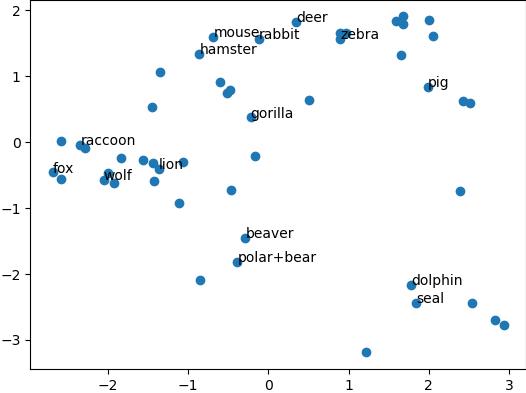
\includegraphics[width = .5\textwidth]{figs/animals_modify.png}
			\caption{Modified Scatter Plot}
		\end{figure}
		\item Which trait of the animals has the largest influence (absolute value) on the first principal component?
		\begin{answer}
			``paws" has the largest influence on the first principal component.
		\end{answer}
		\item Which trait of the animals has the largest influence (absolute value) on the second principal component?
		\begin{answer}
			``vegetation'' has the largest influence on the second principal component.
		\end{answer}
    \end{enumerate}
\end{asking}


\subsection{Data Compression \pts{6}}

It is important to know how much of the information in our dataset is captured by the low-dimensional PCA representation.
In class we discussed the ``analysis'' view that PCA maximizes the variance that is explained by the PCs, and the connection between the Frobenius norm and the variance of a centred data matrix $X$.
Use this connection to answer the following:
\begin{enumerate}
	\item \ask{How much of the variance is explained by our two-dimensional representation from the previous question?}
	\begin{answer}
		With $k = 2$, we have 32\% variance expected without standardization.
	\end{answer}
	\item \ask{How many PCs are required to explain 50\% of the variance in the data?}
	\begin{answer}
	\begin{table}[htbp!]
		\centering
		\begin{tabular}{ll}
			\hline
			Variance Explained & k \\
			\hline
			0.19019081  & 1 \\
			0.32313181  & 2 \\ 
			0.41812272  & 3 \\
			0.48628002  & 4 \\
			0.54465927  & 5 \\
			0.58671039  & 6 \\
			0.62513896  & 7 \\
			0.65789047  & 8 \\
			0.6865892   & 9 \\
			0.71327344  & 10 \\
			\hline
		\end{tabular}
		\caption{Variance Explained}
	\end{table}
	From the table we can see, the variance explained exceeds 50\% when $k \geq 5$.
	\end{answer}
\end{enumerate}
Note: you can compute the Frobenius norm of a matrix using the function \texttt{np.linalg.norm}, among other ways. Also, note that the ``variance explained'' formula from class assumes that $X$ is already centred.


\clearpage
\section{Stochastic Gradient Descent \pts{20}}

If you run \verb|python main.py -q 4|, the program will do the following:
\begin{enumerate}
	\item Load the dynamics learning dataset ($n = 10000, d = 5$)
	\item Standardize the features
	\item Perform gradient descent with line search to optimize an ordinary least squares linear regression model
	\item Report the training error using \texttt{np.mean()}
	\item Produce a learning curve obtained from training
\end{enumerate}

The learning curve obtained from our \texttt{GradientDescentLineSearch} looks like this:
\centerfig{.6}{./figs/gd_line_search_curve.png}

This dataset was generated from a 2D bouncing ball simulation, where the ball is initialized with some random position and random velocity. The ball is released in a box and collides with the sides of the box, while being pulled down by the Earth's gravity. The features of $X$ are the position and the velocity of the ball at some timestep and some irrelevant noise. The label $y$ is the $y$-position of the ball at the next timestep. Your task is to train an ordinary least squares model on this data using stochastic gradient descent instead of the deterministic gradient descent.

\subsection{Batch Size of SGD \pts{5}}

In \texttt{optimizers.py}, you will find \texttt{StochasticGradient}, a \textit{wrapper} class that encapsulates another optimizer--let's call this a base optimizer.
\texttt{StochasticGradient} uses the base optimizer's \texttt{step()} method for each mini-batch to navigate the parameter space.
The constructor for \texttt{StochasticGradient} has two arguments: \texttt{batch\_size} and \texttt{learning\_rate\_getter}. The argument \texttt{learning\_rate\_getter} is an object of class \texttt{LearningRateGetter} which returns the ``current'' value learning rate based on the number of batch-wise gradient descent iterations. Currently. \texttt{ConstantLR} is the only class fully implemented.

\ask{Submit your code} from \texttt{main.py} that instantiates a linear model optimized with \texttt{StochasticGradient} taking \texttt{GradientDescent} (not line search!) as a base optimizer. Do the following:
\begin{enumerate}
		\item Use ordinary least squares objective function (no regularization).
		\item Using \texttt{ConstantLR}, set the step size to $\alpha^t = 0.0003$.
		\item Try the batch size values of $\texttt{batch\_size} \in \{1, 10, 100\}$.
\end{enumerate}
\ask{For each batch size value, use the provided training and validation sets to compute and report training and validation errors after 10 epochs of training. Compare these errors to the error obtained previously.}
\begin{answer}
	With batch size equals to 1, the training error and validation error are both 0.14.

	With batch size equals to 10, the traing error and validation error are both 0.14.

	With batch size equals to 100, the training error is 0.178 and the validation error is 0.177.

	Compare with previous result, where we got training error and validation error both 0.14, we can see that the limit of both errors are 0.14. The errors converge with batch size 1 and 10, but not with batch size 100. Small batch size gives metter results, but at the same time takes more time to compute each iteration.

	\begin{minted}{python}
    loss_fn = LeastSquaresLoss()
    child_optimizer = GradientDescent()
    Learning_rate = ConstantLR(0.0003)
    batch_sizes = [1, 10, 100]

    for i in batch_sizes:
        optimizer = StochasticGradient(child_optimizer, Learning_rate, batch_size= i,max_evals=10)
        model = LinearModel(loss_fn, optimizer, check_correctness=False)
        model.fit(X_train, y_train)
        print(f"Training MSE: {((model.predict(X_train) - y_train) ** 2).mean():.3f}")
        print(f"Validation MSE: {((model.predict(X_val) - y_val) ** 2).mean():.3f}")
	\end{minted}
\end{answer}


\subsection{Learning Rates of SGD \pts{6}}

Implement the other unfinished \texttt{LearningRateGetter} classes, which should return the learning rate $\alpha^t$ based on the following
specifications:
\begin{enumerate}
	\item \texttt{ConstantLR}: $\alpha^t = c$.
	\item \texttt{InverseLR}: $\alpha^t = c/t$.
	\item \texttt{InverseSquaredLR}: $\alpha^t = c/t^2$.
	\item \texttt{InverseSqrtLR}: $\alpha^t = c/\sqrt{t}$.
\end{enumerate}
\ask{Submit your code for these three classes.}

\begin{answer}
	\begin{minted}{python}
	class InverseLR(LearningRateGetter):
		def get_learning_rate(self):
			self.num_evals += 1
			return self.multiplier / self.num_evals

	class InverseSquaredLR(LearningRateGetter):
		def get_learning_rate(self):
			self.num_evals += 1
			return self.multiplier / (self.num_evals **2)

	class InverseSqrtLR(LearningRateGetter):
		def get_learning_rate(self):
			self.num_evals += 1
			return self.multiplier / np.sqrt(self.num_evals)

		
	\end{minted}
\end{answer}

\subsection{The Learning Curves (Again) \pts{9}}

Using the four learning rates, produce a plot of learning curves visualizing the behaviour of the objective function $f$ value on the $y$-axis, and the number of stochastic gradient descent epochs (at least 50) on the $x$-axis. Use a batch size of 10. Use $c = 0.1$ for every learning rate function. \blu{Submit this plot and answer the following question. Which step size functions lead to the parameters converging towards a global minimum?}

\begin{answer}
	\begin{figure}[htbp!]
		\centering
		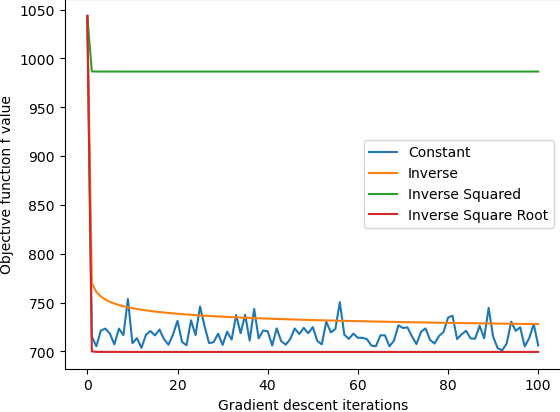
\includegraphics[width = .6\textwidth]{figs/learning_curve.png}
		\caption{Learning Curves}
	\end{figure}

	From the figure, we can see that, the learning curve converges to the minimum with inverse square root step, and converges to a non-optimal point with inverse squared step. It with inverse learning step doesn't converge to the minimum after 100 iterations and might converge to a sub-optimal point. The learning curve with constant step is randomly walking within the range $[700,750]$.
\end{answer}



\clearpage
\section{Very-Short Answer Questions \pts{18}}
\ask{Answer each of the following questions in a sentence or two.}
\begin{enumerate}
\item Assuming we want to use the original features (no change of basis) in a linear model, what is an advantage of the ``other'' normal equations over the original normal equations?
\ans{It's faster when $n << k$.}
\item In class we argued that it's possible to make a kernel version of $k$-means clustering. What would an advantage of kernels be in this context?
\ans{We can find non-convex clusters.}

\item In the language of loss functions and regularization, what is the difference between MLE and MAP?
\ans{MLE doesn't include regularization.}
\item What is the difference between a generative model and a discriminative model?
\ans{Generative models learn the joint distribution, while discriminative models learn the conditionsl distribution. }
\item In this course, we usually add an offset term to a linear model by transforming to a $Z$ with an added constant feature. How can we do that in a kernel model?
\ans{When generating matrix $K$, we add $1$ to each element of the matrix $X_1 * X_2^T$, and then square it. This act is equivalent to adding a constant term in each row ot matrix $Z_i$}

\item With PCA, is it possible for the loss to increase if $k$ is increased? Briefly justify your answer.
\ans{With $k$ larger, we would preserve more information from the original data, so there can't be loss.}


\item Why doesn't it make sense to do PCA with $k > d$?
\ans{Whe we select $k = d$, we are just using the original dataset. If we select $k > d$, we can't gain more information than the original dataset, so it's meaningless. }

\item In terms of the matrices associated with PCA ($X$, $W$, $Z$, $\hat{X}$), where would a single ``eigenface'' be stored?
\ans{Each ``eigenface'' would be a row of $W$}
\item What is an advantage and a disadvantage of using stochastic gradient over SVD when doing PCA?
\ans{An advantage would be a much smaller number of computation in each iteration, and at the same time, it might take more iterations to converge to the minimum, or might even converge into a non-optimal point. }
\end{enumerate}
\end{document}
